% !TEX = root../thesis.tex

\chapter{Real Time Muon Reconstruction at the Compact Muon Solenoid}
\label{chap:kbmtf}

\section{Introduction} \label{sec:kbmtf_intro}
Section~\ref{sec:CMS_L1T} provides an overview of the L1 trigger and its importance to the CMS trigger system. This section will detail the design and performance of a Kalman Filter algorithm used to identify muon tracks in the barrel region of the CMS detector. This algorithm, known as the Kalman Barrel Muon Track Finder (KBMTF), was fully implemented for 2018 data taking and received improvements for continued use in Run-3.

\section{The Kalman Filter Algorithm} \label{sec:kalman_filter}
A Kalman Filter is a tracking algorithm that effectively performs a recursive, iterative chi-squared fit. Qualitatively, it propagates a system from its current state to the next and combines the predicted value with measurements to "update" the state of the system. This updated system can then be propagated and combined with new measured values. This section deals specifically with a discrete linear Kalman Filter, which is applicable when a system can be described with a vector of variables whose evolution can be modeled with a linear transformation plus random uncertainties~\cite{FRUHWIRTH1987444}.

Abstractly, the state of a system at a given step $n-1$ can be described by a vector labeled $x_{n-1}$ with covariance matrix $P_{n-1}$. Let the matrix $F_n$ represent the linear transformation that propagates $x_{n-1}$ to the next state $x_{n}$, and the matrix $Q_{n}$ be the covariance matrix due to random uncertainty. The predicted state of the system at step $n$ can be given by
\begin{equation}
	\label{eq:prop}
	x_{n}=F_{n}x_{n-1} \quad \textrm{and} \quad P_{n}=F_nP_{n-1}F_n^T+Q_n
\end{equation}

Now define a set of measurements taken at state $n$ as $z_n$ with covariance matrix $R_n$. The measured variables are not restricted to the same set of variables defining $x_n$ as long as there exist a change of basis matrix $H$ that relates the sets. The predicted state and covariance matrix of the system written in the same basis as the measured quantities is defined as
\begin{equation}
	\label{eq:changeOfBasis}
	\mu_n\coloneqq Hx_n \quad \textrm{and} \quad \Sigma_n\coloneqq HP_nH^{T}
\end{equation}

Updating the system relies on a matrix known as the Kalman Gain, which acts as a weight based on $\Sigma_n$ and $R_n$ and effectively determines if the updated system should skew more towards the measured or predicted values. The Kalman gain is defined as
\begin{equation}
	\label{eq:gain}
	K\coloneqq \Sigma_n\left(\Sigma_n+R_n\right)^{-1}
\end{equation}

The Kalman gain is then used to calculate the updated system as follows
\begin{equation}
	\label{eq:update1}
	\mu_n'=\mu_n+K\left(z_n-\mu_n\right) \quad \textrm{and} \quad \Sigma_n'=\Sigma_n-K\Sigma_n
\end{equation}

A kalman gain equal to the identity $I$ would set the updated coordinates to the measured values, while a kalman gain of $0$ would effectively ignore the measured values. Finally, the system is transformed back to the original variables used in the prediction, at which stage the process can be repeated to evolve the system to state $n+1$.
\begin{equation}
	x_n'=x_n+H^TK(z_n-\mu_n) \quad \mathrm{and} \quad P_n'= P_n-H^TKHP_n
\end{equation}

\subsection{Muon Trajectory Propagation} \label{sec:muons_prop}
The passage of charged particles through magnetic fields is well understood from the Lorentz Force Law. Using the geometry described in section~\ref{sec:CMS_coord}, a particle with charge $q$ and transverse momentum travels in a circular trajectory with radius $R$ when viewed in the $r$-$\varphi$ plane. These can be related by $p_{T} = qBR$. In particle physics, when working with an object of elementary charge, this is commonly rewritten as
\begin{equation}
	\label{eq:pt03br}
	p_{T} = 0.3BR\unit{[GeV/c]}
\end{equation} 

With the high center of mass energy, the radius of these trajectories is substantially smaller than the size of the CMS detector. Assuming a coordinate system with the particle starting at the origin, the circular trajectory can be approximated using a parabola as
\begin{equation}
	\label{eq:parabola1}
	y(x)=\frac{x^2}{2R}+bx
\end{equation}
where $b$ is a coefficient depending on the orientation of the coordinate system. If the initial trajectory is defined as $\phi_{b,0}$, taking the derivative and evaluating at the origin yields
\begin{equation}
	\label{eq:phib}
	y'(0)=\tan(\phi_{b,0})=b
\end{equation}	
The curvature $k=q/p_{T}$ is the preferred variable to work with when propagating the trajectory of a muon, as the propagation is linear in $k$. This along with equations~\ref{eq:pt03br}-\ref{eq:phib} and combining constant coefficients of x yields
\begin{equation}
	\label{eq:parabola2}
	y(x)=akx^2+\tan(\phi_{b,0})x
\end{equation}

Muon hits (or "stubs") provide information on the position $\phi$ and bending angle $\phi_b$. Define the radius of two sequential muon stations as $r_1$ and $r_2$, with the outer radius given by $r_2$ and $\Delta r=r_2-r_1$. Assuming a muon has curvature $k$ at the outer station and negligible energy loss, equation~\ref{eq:parabola2} can be used to propagate stubs from the outer station towards the inner station.
\begin{equation}
	y(-\Delta r) = \left(a\Delta r^2\right)k-\Delta r\tan(\phi_{b,0})
\end{equation}
\begin{equation}
	y'(-\Delta r)=-\left(2a\Delta r\right)k+\tan(\phi_{b,0})
\end{equation}
Converting these to the quantities to angles yields
\begin{equation}
	\label{eq:prop_phi}
	\sin(\Delta\phi)\approx\Delta\phi=\frac{y(-\Delta r)}{r_1} = \frac{a\Delta r^2}{r_1}k-\frac{\Delta r}{r_1}\phi_{b,0}
\end{equation}
\begin{equation}
	\label{eq:prop_phib}
	\phi_b=\Delta\phi+\mathrm{tan}^{-1}\left[y'(-\Delta r)\right]\approx a\Delta r\left(\frac{\Delta r}{r_1}-2\right)k+\left(\frac{r_2}{r_1}\right)\phi_{b,0}
\end{equation}
Where we have used the small angle approximation to simplify $\sin(x)$, $\tan(x)$, and $\mathrm{tan}^{-1}(x)$ as $\sim x$ in order to express the propagated coordinates as a linear combination of the initial curvature $k$, position $\phi$, and bending angle $\phi_{b,0}$. The $\Delta\phi$ term is added to equation~\ref{eq:prop_phib} because the bending angle at each station is measured relative to an axis system oriented towards the center of the detector. A diagram showing this propagation can be seen in figure~\ref{fig:mu_trajectory}.

\begin{figure}[h!]
	\centering
	%Final image: origin at outer stub, oriented with x axis pointing towards vertex
	\begin{tikzpicture}
		% axis system
		\draw[thick,->] (-11, 0) -- (1, 0) node[anchor=west] {x};
		\draw[thick,->] (0, 0) -- (0, 4) node[anchor=south east] {y};
		\coordinate[label = above left:$\mathrm{Vertex}$] (vertex) at (-9.5, 0);
		\coordinate[label = above right:$\mathrm{Origin}$] (origin) at (0, 0);
		\coordinate[] (r1) at (-5, 0);
		\node at (vertex)[circle,fill,inner sep=2pt]{};
		\node at (origin)[circle,fill,inner sep=2pt]{};
		\draw[<->] (-9.5, -.5) -- (-5, -.5);
		\draw[<->] (-9.5, -1.1) -- (0, -1.1);
		\coordinate[label = below:$r_1$] (r1) at (-7.25,-.5);
		\coordinate[label = below:$r_2$] (r2) at (-5,-1.1);
		\draw[dashed] (-5, 0) -- (-5, 4);
		
		% muon trajectory
		\def \X{2.6047227}; %circle x0
		\def \Y{14.772116}; %circle y0
		\def \sy{1.8427620};%stub at (-5, y)
		\draw [<-, domain=270:230] plot ({\X+15*cos(\x)}, {\Y+15*sin(\x)});
		\draw (-2.25,.25) node[anchor=west] {$\phi_{b,0}$};
		\coordinate[] (stub1) at (-5, \sy);
		\draw [dashed, domain=0:6] plot ({-9.5+\x}, {0.40950267*\x});
		\draw [dashed] (-5, \sy) -- (-4, \sy);
		\draw (-8.5, .25) node[anchor=west] {$\Delta\phi$};
		\draw (-4, \sy) node[anchor=west, scale=1.0] {$\phi_b$};
		\draw (-4.5, \sy+.1) node[anchor=west, scale=0.7] {$\Delta\phi$};
	\end{tikzpicture}
	\caption{Diagram showing a muon trajectory between two stations with the origin set at the outer station. The x-axis is oriented using the detector vertex and the outer station.}
	\label{fig:mu_trajectory}
\end{figure}

\subsection{Implementation of the Kalman Barrel Muon Track Finder} \label{sec:kbmtf}
Muon track finding begins from the outer chambers and propagates inward because the outermost chambers are the lowest occupancy, as background events are more likely to be stopped as they travel through more material. A rough outline KBMTF algorithm for track finding is as follows:
\begin{enumerate}
	\item A track seed is chosen from stubs in the muon station, which provides a preliminary track with $k$, $\phi$, and $\phi_{b}$. This seed cannot be chosen from the innermost muon station. \label{kbmtf_step1}
	\item If the track is not at the innermost station, the track is propagated inward to the next station. \label{kbmtf_step2}
	\item Stubs in the inner station are matched to the propagated track. \label{kbmtf_step3}
	\begin{itemize}
		\item If there are matching stubs, pick the best most similar in $\phi$ and $\phi_b$ and create an updated track using the stub information
	\end{itemize}
	\item Repeat steps~\ref{kbmtf_step2}-\ref{kbmtf_step3} until the track is at the innermost station
	\item Propagate the track from the innermost station to the vertex
	\begin{itemize}
		\item The $d_{xy}$ of the track is defined as the closest distance from this propagated track to the vertex, and the track values are stored as the "vertex unconstrained" measurement.
	\end{itemize} \label{kbmtf_step4}
	\item The vertex propagated track is updated with the constraint that the track originated from the beamline, known as the "vertex constrained" measurement. \label{kbmtf_step5}
\end{enumerate}

Tracks are then overlap cleaned, which ensures that stubs are not shared between multiple tracks, and cut based on various goodness of fit criteria. A diagram showing the KBMTF propagation and update procedure can be shown in figure~\ref{fig:kbmtf}.

\begin{figure} [htb!]
	\centering
	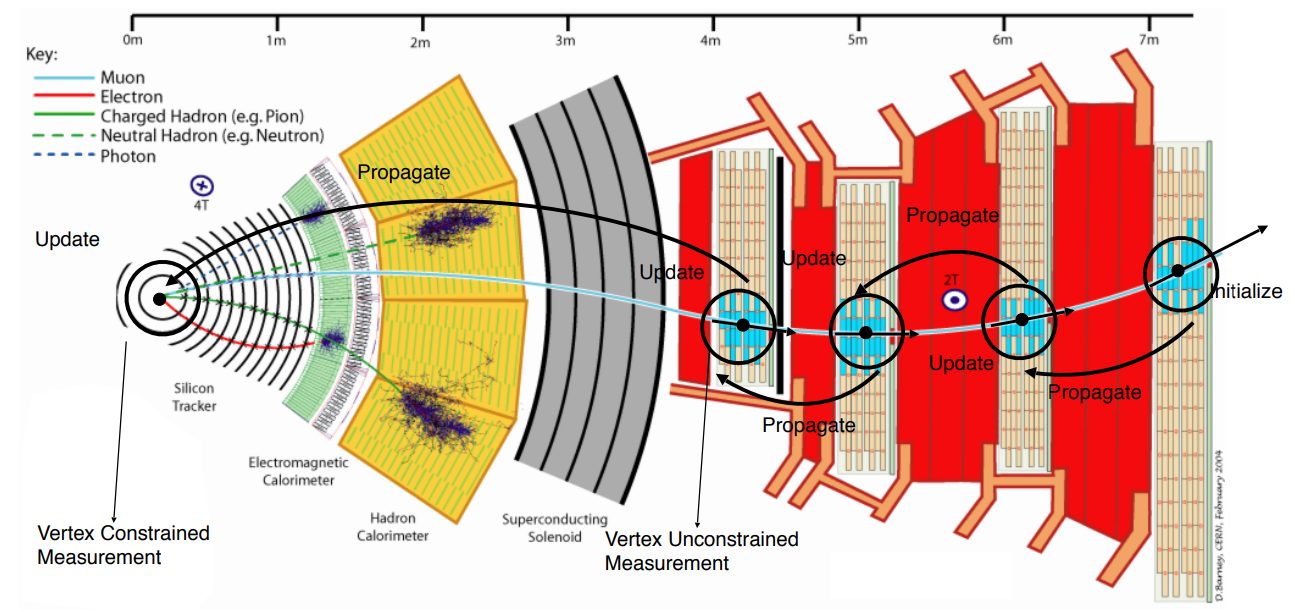
\includegraphics[width=0.85\linewidth]{figs/04_muons/kbmtf_diagram.png}
	\caption[The iterative process of propagation and updating a muon track through the KBMTF algorithm. The track properties at the innermost station are stored in order to trigger on muons not originating from the beamline~\cite{CERN-LHCC-2020-004}]
	{The iterative process of propagation and updating a muon track through the KBMTF algorithm. The track properties at the innermost station are stored in order to trigger on muons not originating from the beamline~\cite{CERN-LHCC-2020-004}.}
	\label{fig:kbmtf}
\end{figure}

\subsubsection{Track propagation}\label{sec:kbmtf_prop}
Equations~\ref{eq:prop_phi}-\ref{eq:prop_phib} show that the track propagation fits the criteria for a discrete linear Kalman Filter discussed in section~\ref{sec:kalman_filter}. The matrices can now be constructed as follows. The transfer matrix $F_n$ from equation~\ref{eq:prop} can be expressed as
\begin{equation}
	\label{eq:kmtfProp}
	x_{n}=\left(\begin{matrix}
		k\\
		\phi\\
		\phi_b
	\end{matrix}\right)_{n} = 
\left(\begin{matrix}
	1 & 0 & 0\\
	\alpha_n & 1 & -\frac{\Delta r}{r_n}\\
	\beta_n & 0 & \frac{r_{n-1}}{r_n}
\end{matrix}\right)
\left(\begin{matrix}
	k\\
	\phi\\
	\phi_b
\end{matrix}\right)_{n-1}=F_nx_{n-1}
\end{equation}
where the coefficients
\begin{equation}
	\label{eq:kmtf_coeff}
	\alpha_n=a\frac{\Delta r^2}{r_n} \quad \mathrm{and} \quad \beta_n=a\Delta r\left(\frac{\Delta r}{r_n}-2\right)
\end{equation}
with $r_{n-1}$ being the radius of the previous (outer) muon station and $r_n$ the radius of the sequential (inner) muon station. Since the muon detectors only measure $\phi$ and $\phi_b$, the matrix $H$ described in equation~\ref{eq:changeOfBasis} must be a 2$\times$3 matrix that takes the form
\begin{equation}
	H=\left(\begin{matrix}
		0 & 1 & 0\\
		0 & 0 & 1\end{matrix}\right)
\end{equation}

While the radii of the muon stations are determined by detector geometry, the constants $\alpha_n$ and $\beta_n$ are measured using single muon monte-carlo samples where stubs are matched to the incident muons using generator level information. To determine $\alpha_n$, stubs in stations $n$ and $n-1$ are associated if they resulted from the same incident muon. For matching stubs, the quantity $\Delta\phi+\frac{\Delta r}{r_1}\phi_{b,0}$ is plotted versus the muon $k$ in a 2-dimensional histogram. Slices along the y-axis are fit using a Gaussian distribution, and the mean value for each slice is used to calculate a linear fit as a function of $k$. $\beta_n$ is calculated similarly by plotting $\phi_b-\left(r_{n-1}/r_n\right)\phi_{b,0}$ vs $k$.

\subsubsection{Covariant Matrices} \label{sec:kbmtf_cov}
There are two sources of uncertainty that affect the covariance matrices. The first is multiple coulomb scattering, which occurs when muons scatter elastically with material in the detector. This can be thought of as a small "kick" in momentum that deflects the muon. Lower momentum muons will be deflected at greater angles, so this uncertainty is proportional to $k$. Additionally, the probability for multiple scattering is proportional to the amount of material traversed by the muon, so this uncertainty must be calculated for each step in propagation. The second source is from the intrinsic detector resolution, which is a fixed value for each detector. However, the angular resolution is dependent on the radial distance from the center of the detector, so these must be calculated for each station as well. The uncertainty resulting from both of these factors is given by
\begin{equation}
	\label{eq:prop_uncertainty}
	\sigma(k)=\sqrt{\sigma_{ms}^2k^2+\sigma_{res}^2}
\end{equation}

The coefficients can be calculated by using the Gaussian slice fits described when deriving $\alpha$ and $\beta$. For each propagation, the sigma of the Gaussian fits is plotted vs $k$ and fit to the form in equation~\ref{eq:prop_uncertainty}. This fitting process for $\phi$ propagation coefficients is shown in figure~\ref{fig:phi_prop}.

\begin{figure}[htb!]
	\centering
	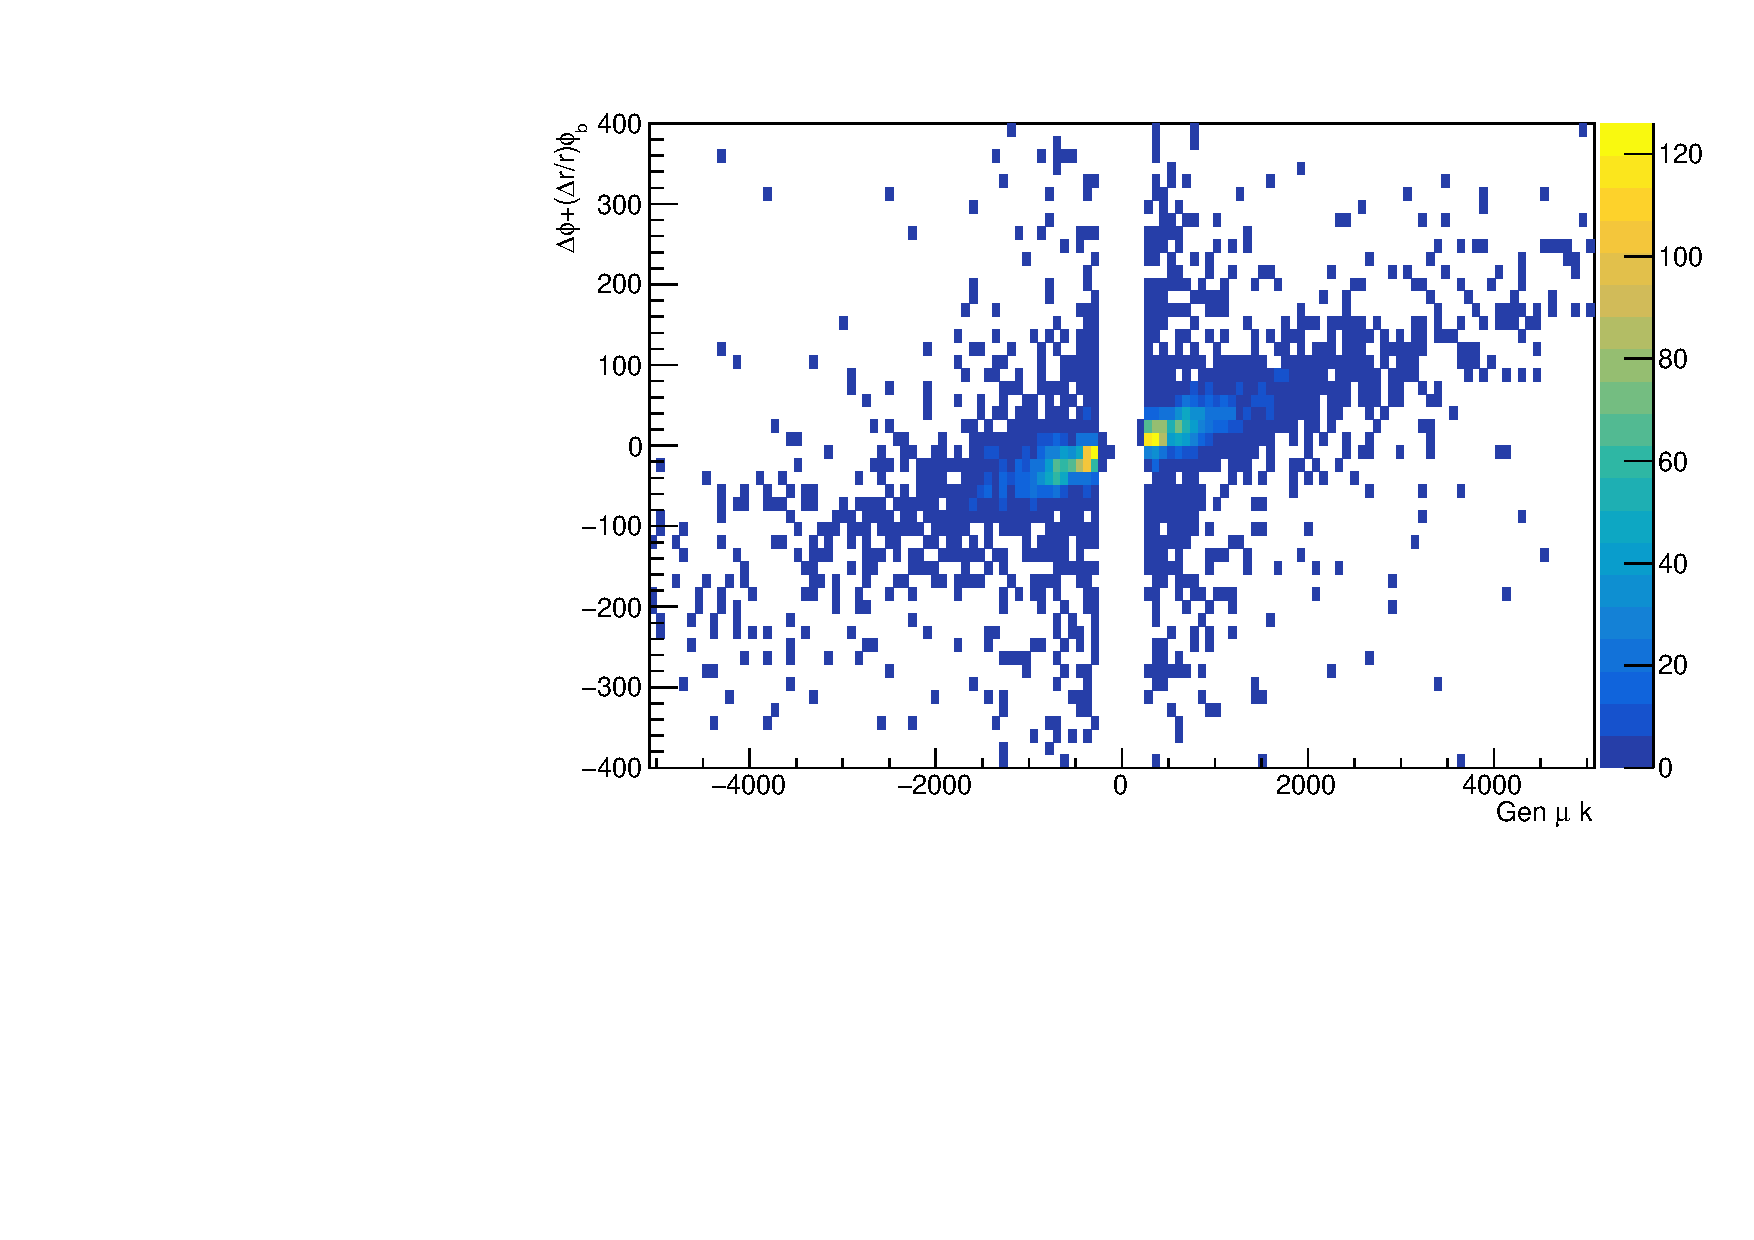
\includegraphics[width=0.32\linewidth]{figs/04_muons/phiprop_2d.pdf}
	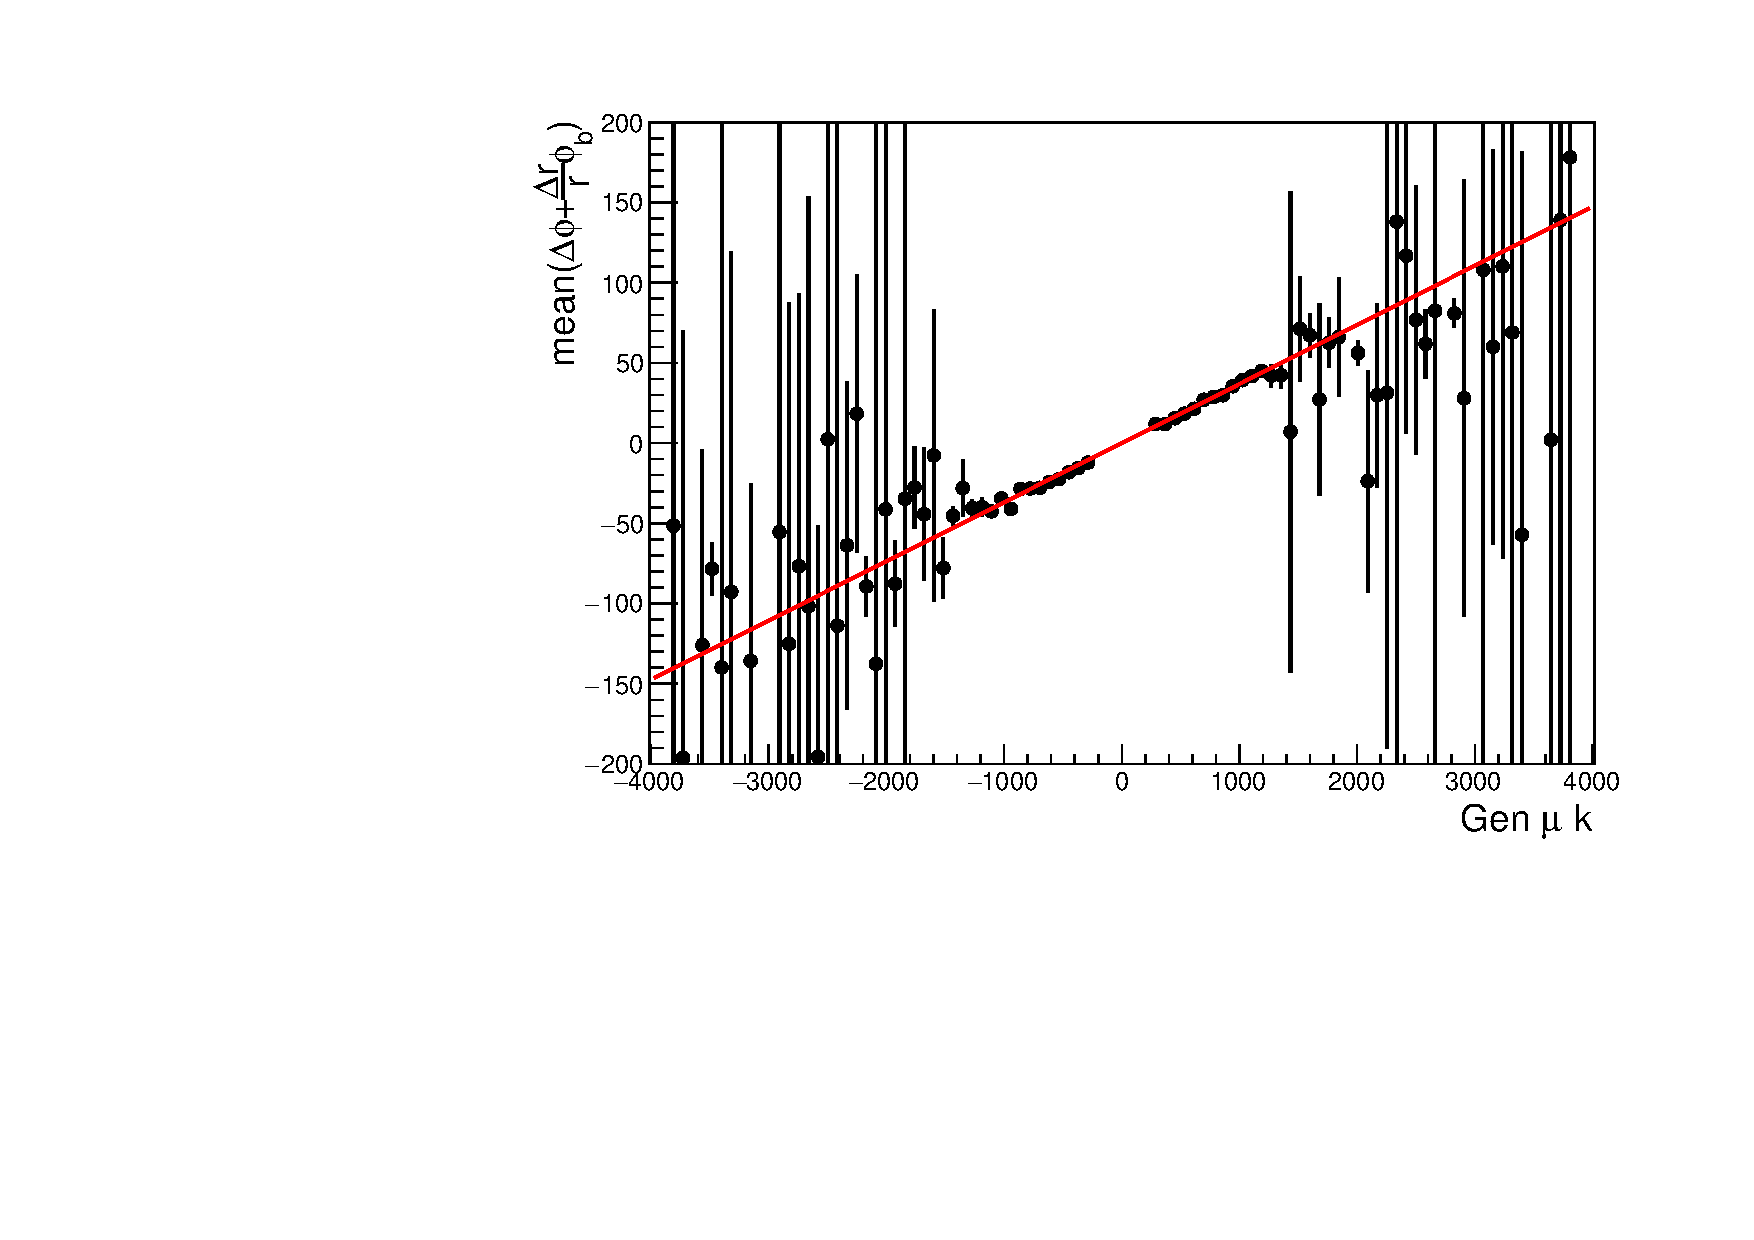
\includegraphics[width=0.32\linewidth]{figs/04_muons/phiprop_mean.pdf}
	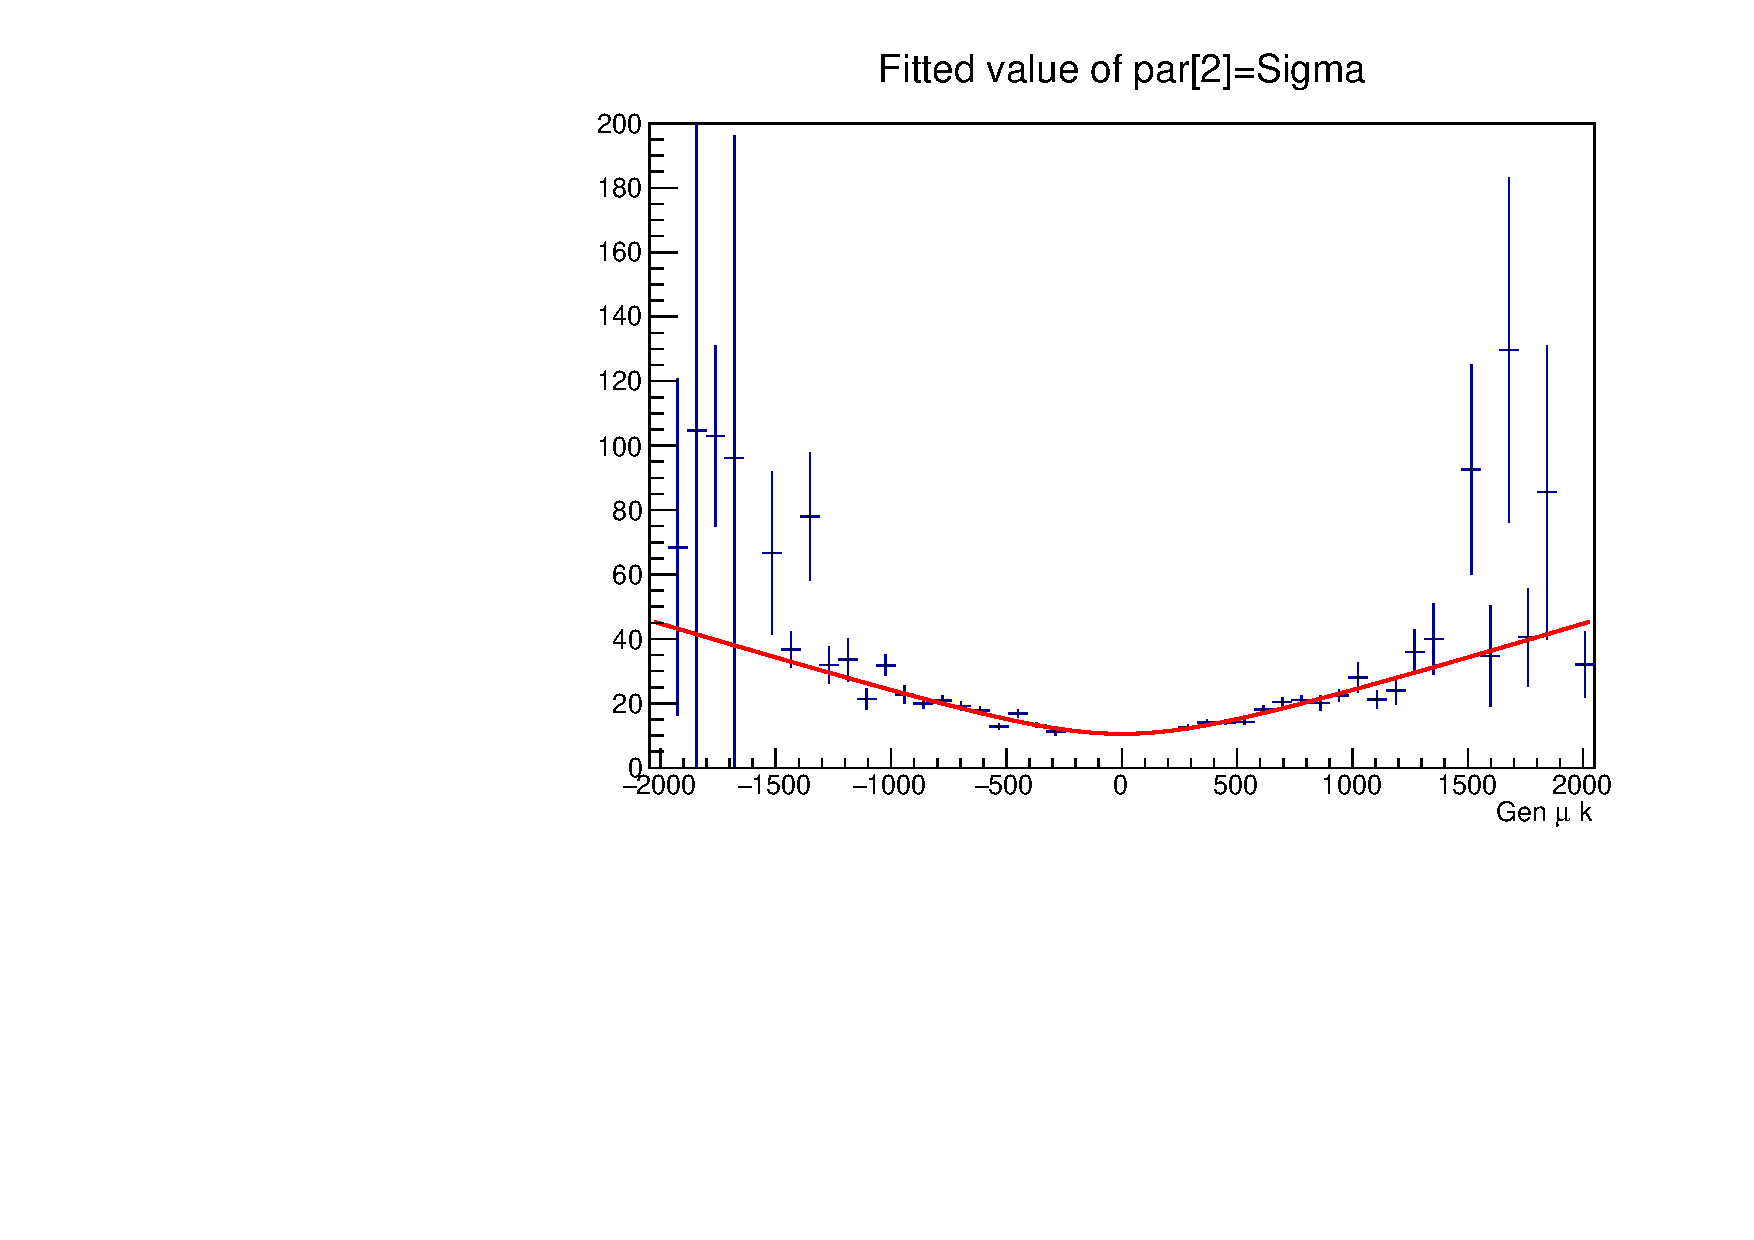
\includegraphics[width=0.32\linewidth]{figs/04_muons/phiprop_sigma.pdf}
	\caption[Calculation of phi propagation coefficients. Units are converted to their digitized form used in firmware calculation. (Left) 2-dimension histogram of $\Delta\phi+\frac{\Delta r}{r_1}\phi_{b,0}$ vs $k$. (Center) Mean of vertical slices fits used to calculate $\alpha$. (Right) Sigma of vertical slices used to calculate multiple scattering and resolution uncertainties.]
	{Calculation of phi propagation coefficients. Units are converted to their digitized form used in firmware calculation. (Left) 2-dimension histogram of $\Delta\phi+\frac{\Delta r}{r_1}\phi_{b,0}$ vs $k$. (Center) Mean of vertical slices fits used to calculate $\alpha$. (Right) Sigma of vertical slices used to calculate multiple scattering and resolution uncertainties.}
	\label{fig:phi_prop}
\end{figure}

In practice, the detector $\phi$ measurements are substantially more precise and have much lower uncertainty than the propagated values.

\subsubsection{Kalman Gain} \label{sec:kbmtf_gain}
The kalman gain described in equation~\ref{eq:gain} can be calculated exactly given the multiple scattering and position resolution coefficients. However, matrix inversion requires division, which in hardware is not computationally viable due to the latency requirements. Instead, an approximate value of the kalman gain is stored in lookup tables as a function of track pattern and muon curvature.